\documentclass[10pt]{article}
\usepackage[landscape,margin=0.6in]{geometry}
\usepackage[T1]{fontenc}
\usepackage{tikz}
\usepackage{hyperref}

\pagestyle{empty}

% Horizontal positions of the four lifelines (cm)
\def\xB{0}\def\xA{7}\def\xD{14}\def\xS{21}

\tikzset{
  participant/.style={draw, rounded corners, fill=blue!7,
    minimum width=3.1cm, minimum height=0.8cm, align=center, font=\small},
  lifeline/.style={draw, dashed, gray},
  call/.style={->, thick},
  reply/.style={->, thick, dashed},
  label/.style={font=\scriptsize, align=center, fill=white, inner sep=2pt},
  phase/.style={font=\small\bfseries, fill=blue!10, rounded corners,
    minimum width=24.1cm, minimum height=0.55cm, align=left, inner xsep=6pt,
    anchor=west},
  note/.style={draw, rounded corners, fill=yellow!15, font=\scriptsize,
    align=center, inner sep=3pt}
}

% \header{lifeline length}
\newcommand{\header}[1]{%
  \node[participant] (browser) at (\xB,0) {User / Browser\\Next.js client};
  \node[participant] (api) at (\xA,0) {Fastify API\\(via Next.js \texttt{/api} proxy)};
  \node[participant] (db) at (\xD,0) {PostgreSQL};
  \node[participant] (storage) at (\xS,0) {Shared roots\\(\texttt{SHARED\_FOLDERS} mounts)};
  \foreach \x in {\xB,\xA,\xD,\xS}
    \draw[lifeline] (\x,-0.5) -- (\x,-#1);
}

\begin{document}

%%%%%%%%%%%%%%%%%%%%%%%%%%%%%%%%%%%%%%%%%%%%%%%%%%%%%%%%%%%%%%%%%%%%%%%%
% PAGE 1
%%%%%%%%%%%%%%%%%%%%%%%%%%%%%%%%%%%%%%%%%%%%%%%%%%%%%%%%%%%%%%%%%%%%%%%%
\begin{center}
  {\Large\bfseries Mizore: current application sequence}\\[2pt]
  {\small Main user journey: sign in, load saved paths, add a path, and browse files}
\end{center}
\vspace{-1mm}

\begin{center}
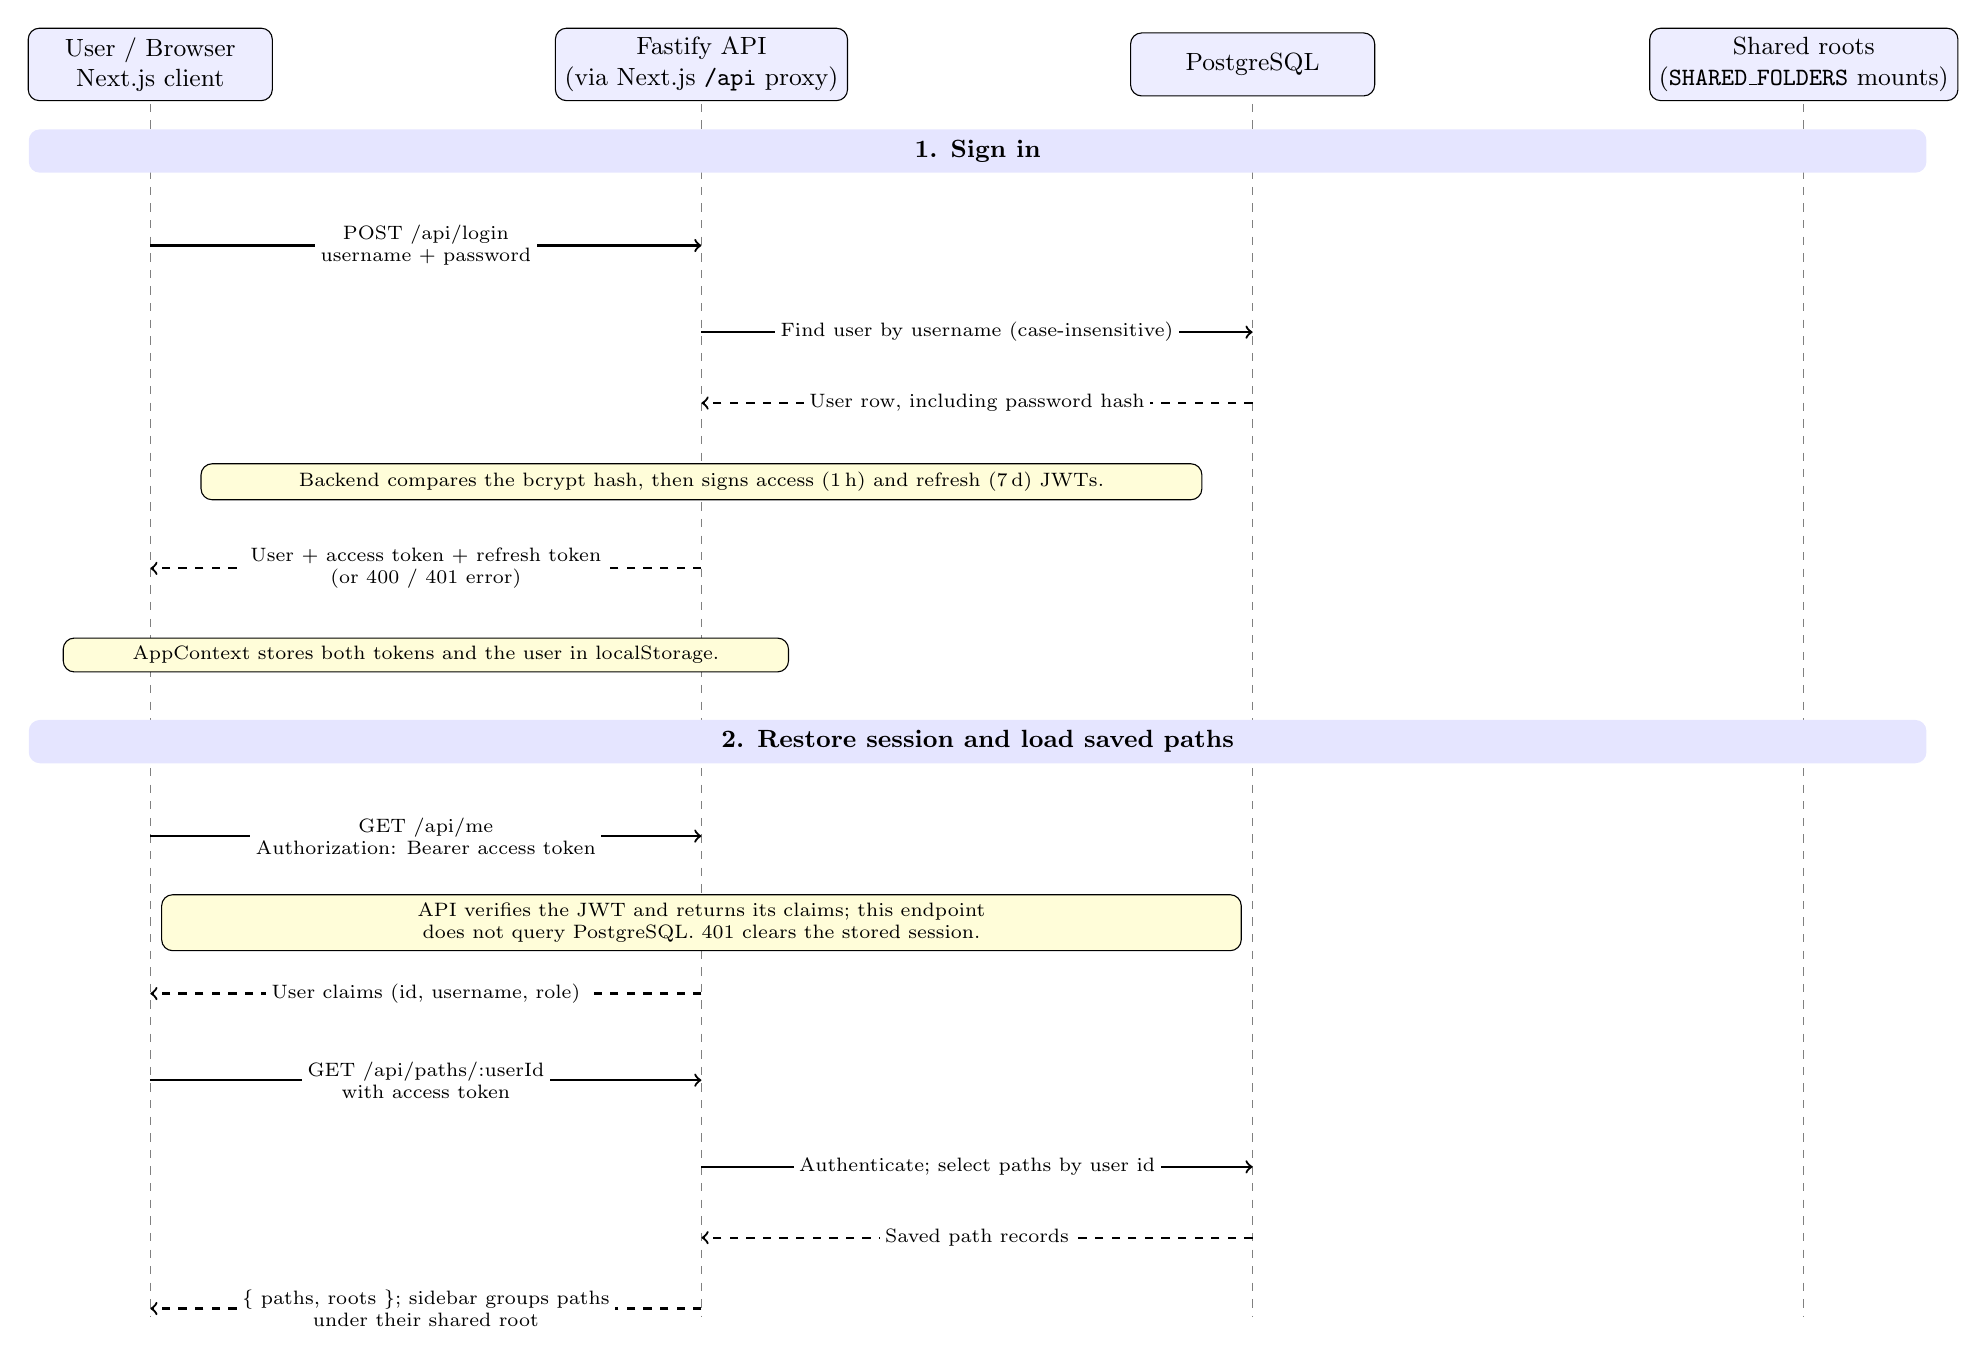
\begin{tikzpicture}
\header{15.9}

% 1. Sign in
\node[phase] at (-1.55,-1.1) {1. Sign in};
\draw[call] (\xB,-2.3) -- (\xA,-2.3)
  node[midway,label] {POST /api/login\\username + password};
\draw[call] (\xA,-3.4) -- (\xD,-3.4)
  node[midway,label] {Find user by username (case-insensitive)};
\draw[reply] (\xD,-4.3) -- (\xA,-4.3)
  node[midway,label] {User row, including password hash};
\node[note,text width=12.5cm] at (\xA,-5.3)
  {Backend compares the bcrypt hash, then signs access (1\,h) and refresh (7\,d) JWTs.};
\draw[reply] (\xA,-6.4) -- (\xB,-6.4)
  node[midway,label] {User + access token + refresh token\\(or 400 / 401 error)};
\node[note,text width=9cm] at (\xB+3.5,-7.5)
  {AppContext stores both tokens and the user in localStorage.};

% 2. Restore session and load saved paths
\node[phase] at (-1.55,-8.6) {2. Restore session and load saved paths};
\draw[call] (\xB,-9.8) -- (\xA,-9.8)
  node[midway,label] {GET /api/me\\Authorization: Bearer access token};
\node[note,text width=13.5cm] at (\xA,-10.9)
  {API verifies the JWT and returns its claims; this endpoint does not query PostgreSQL. 401 clears the stored session.};
\draw[reply] (\xA,-11.8) -- (\xB,-11.8)
  node[midway,label] {User claims (id, username, role)};
\draw[call] (\xB,-12.9) -- (\xA,-12.9)
  node[midway,label] {GET /api/paths/:userId\\with access token};
\draw[call] (\xA,-14.0) -- (\xD,-14.0)
  node[midway,label] {Authenticate; select paths by user id};
\draw[reply] (\xD,-14.9) -- (\xA,-14.9)
  node[midway,label] {Saved path records};
\draw[reply] (\xA,-15.8) -- (\xB,-15.8)
  node[midway,label] {\{ paths, roots \}; sidebar groups paths\\under their shared root};
\end{tikzpicture}
\end{center}

\newpage
%%%%%%%%%%%%%%%%%%%%%%%%%%%%%%%%%%%%%%%%%%%%%%%%%%%%%%%%%%%%%%%%%%%%%%%%
% PAGE 2
%%%%%%%%%%%%%%%%%%%%%%%%%%%%%%%%%%%%%%%%%%%%%%%%%%%%%%%%%%%%%%%%%%%%%%%%
\begin{center}
  {\large\bfseries Mizore: current application sequence (continued)}
\end{center}
\vspace{-1mm}

\begin{center}
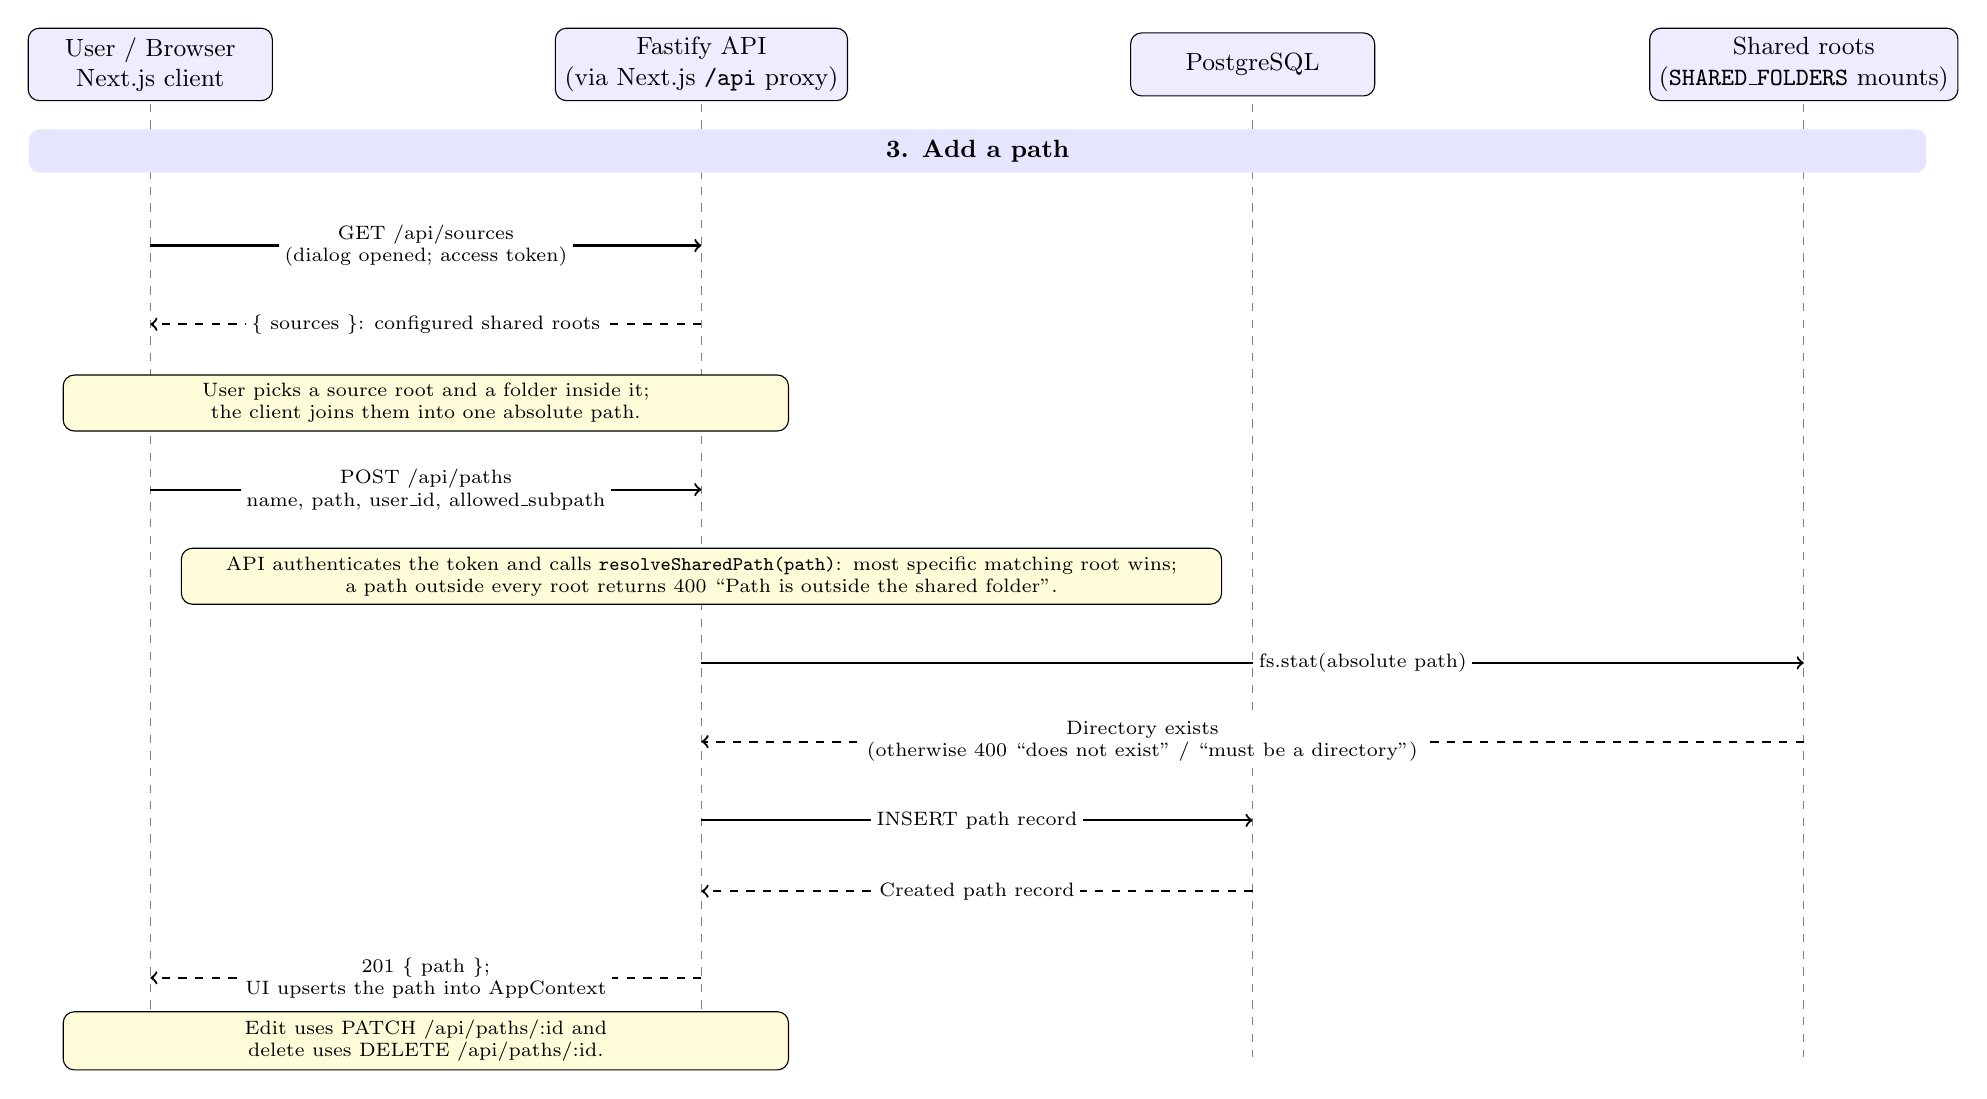
\begin{tikzpicture}
\header{12.6}

% 3. Add a path
\node[phase] at (-1.55,-1.1) {3. Add a path};
\draw[call] (\xB,-2.3) -- (\xA,-2.3)
  node[midway,label] {GET /api/sources\\(dialog opened; access token)};
\draw[reply] (\xA,-3.3) -- (\xB,-3.3)
  node[midway,label] {\{ sources \}: configured shared roots};
\node[note,text width=9cm] at (\xB+3.5,-4.3)
  {User picks a source root and a folder inside it; the client joins them into one absolute path.};
\draw[call] (\xB,-5.4) -- (\xA,-5.4)
  node[midway,label] {POST /api/paths\\name, path, user\_id, allowed\_subpath};
\node[note,text width=13cm] at (\xA,-6.5)
  {API authenticates the token and calls \texttt{resolveSharedPath(path)}: most specific matching root wins;\\
   a path outside every root returns 400 ``Path is outside the shared folder''.};
\draw[call] (\xA,-7.6) -- (\xS,-7.6)
  node[pos=0.6,label] {fs.stat(absolute path)};
\draw[reply] (\xS,-8.6) -- (\xA,-8.6)
  node[pos=0.6,label] {Directory exists\\(otherwise 400 ``does not exist'' / ``must be a directory'')};
\draw[call] (\xA,-9.6) -- (\xD,-9.6)
  node[midway,label] {INSERT path record};
\draw[reply] (\xD,-10.5) -- (\xA,-10.5)
  node[midway,label] {Created path record};
\draw[reply] (\xA,-11.6) -- (\xB,-11.6)
  node[midway,label] {201 \{ path \};\\UI upserts the path into AppContext};
\node[note,text width=9cm] at (\xB+3.5,-12.4)
  {Edit uses PATCH /api/paths/:id and delete uses DELETE /api/paths/:id.};
\end{tikzpicture}
\end{center}

\newpage
%%%%%%%%%%%%%%%%%%%%%%%%%%%%%%%%%%%%%%%%%%%%%%%%%%%%%%%%%%%%%%%%%%%%%%%%
% PAGE 3
%%%%%%%%%%%%%%%%%%%%%%%%%%%%%%%%%%%%%%%%%%%%%%%%%%%%%%%%%%%%%%%%%%%%%%%%
\begin{center}
  {\large\bfseries Mizore: current application sequence (continued)}
\end{center}
\vspace{-1mm}

\begin{center}
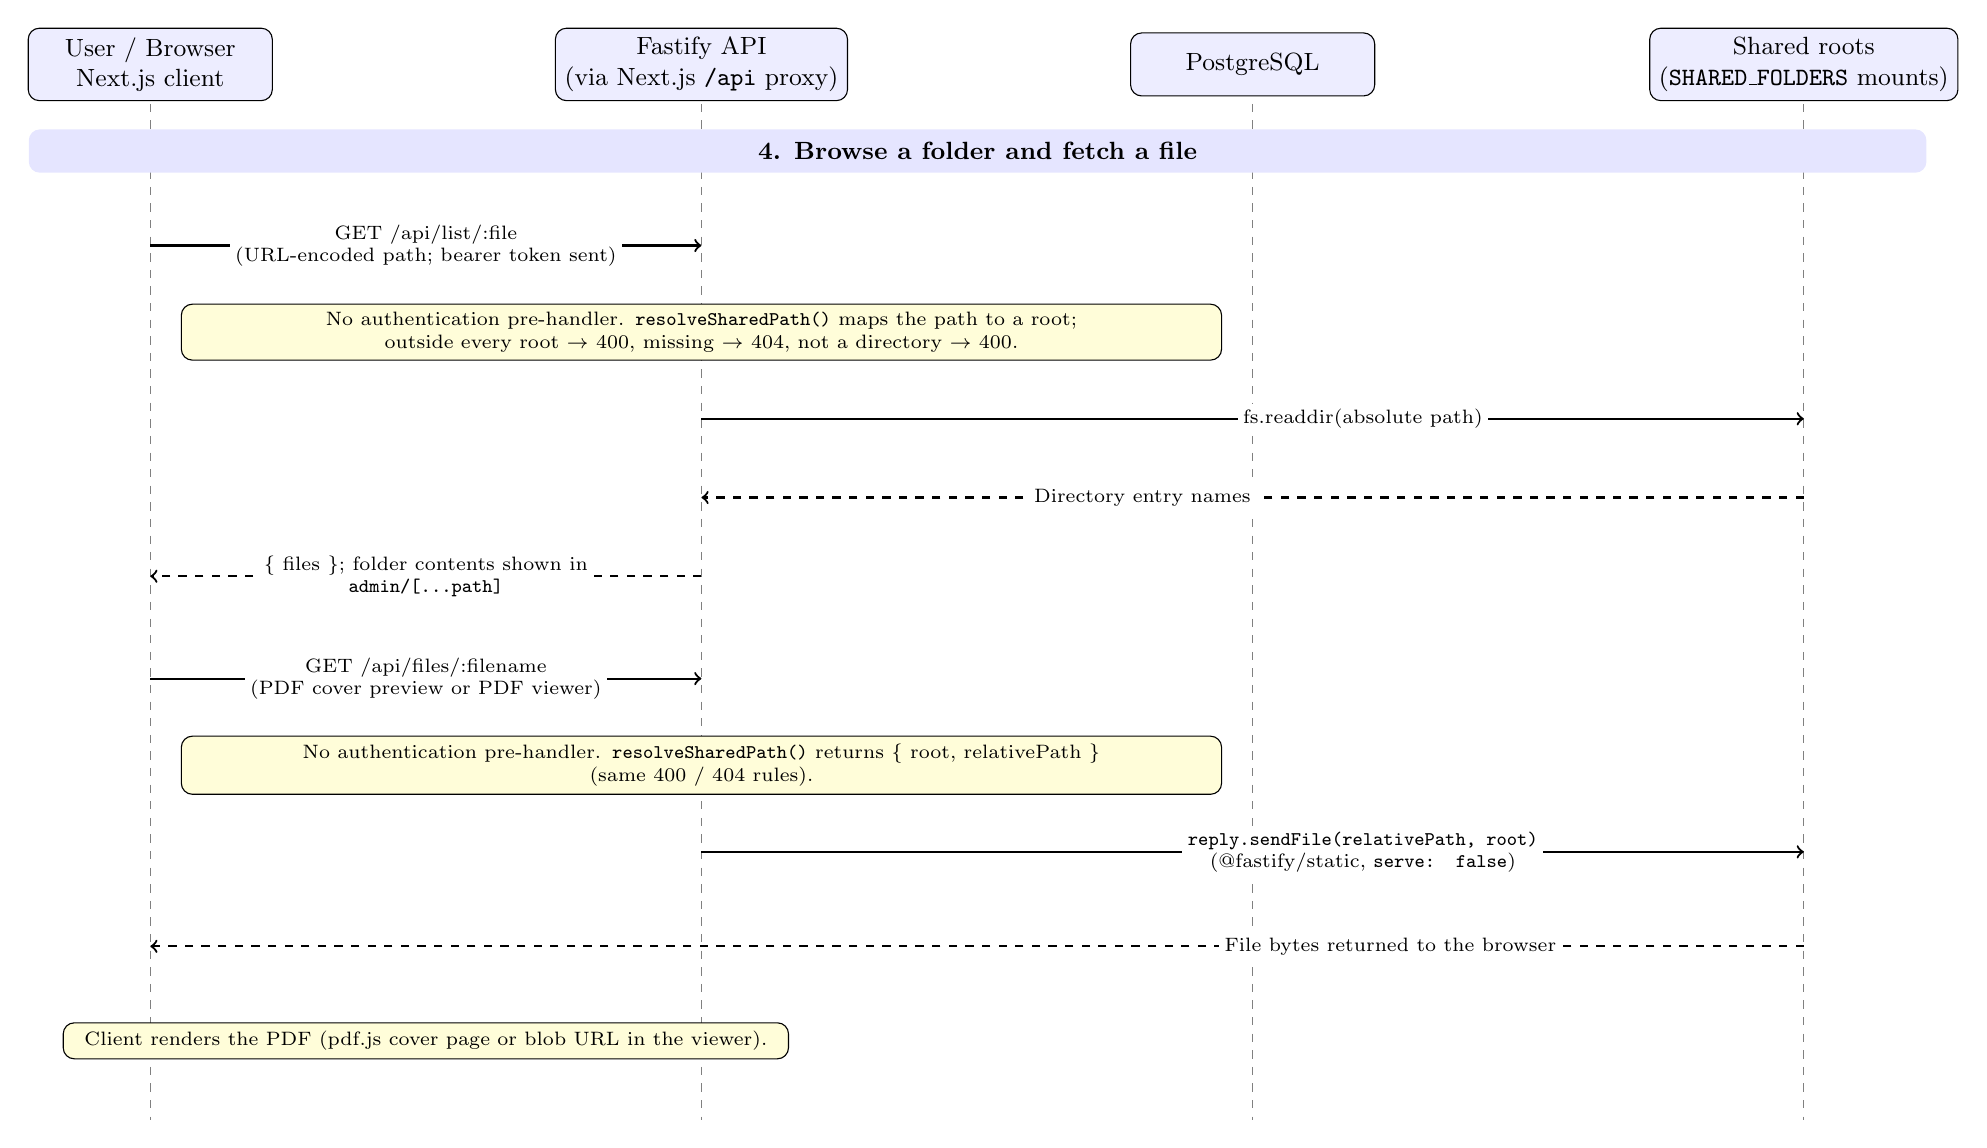
\begin{tikzpicture}
\header{13.4}

% 4. Browse a folder and fetch a file
\node[phase] at (-1.55,-1.1) {4. Browse a folder and fetch a file};
\draw[call] (\xB,-2.3) -- (\xA,-2.3)
  node[midway,label] {GET /api/list/:file\\(URL-encoded path; bearer token sent)};
\node[note,text width=13cm] at (\xA,-3.4)
  {No authentication pre-handler. \texttt{resolveSharedPath()} maps the path to a root;\\
   outside every root $\rightarrow$ 400, missing $\rightarrow$ 404, not a directory $\rightarrow$ 400.};
\draw[call] (\xA,-4.5) -- (\xS,-4.5)
  node[pos=0.6,label] {fs.readdir(absolute path)};
\draw[reply] (\xS,-5.5) -- (\xA,-5.5)
  node[pos=0.6,label] {Directory entry names};
\draw[reply] (\xA,-6.5) -- (\xB,-6.5)
  node[midway,label] {\{ files \}; folder contents shown in\\\texttt{admin/[...path]}};
\draw[call] (\xB,-7.8) -- (\xA,-7.8)
  node[midway,label] {GET /api/files/:filename\\(PDF cover preview or PDF viewer)};
\node[note,text width=13cm] at (\xA,-8.9)
  {No authentication pre-handler. \texttt{resolveSharedPath()} returns \{ root, relativePath \}\\
   (same 400 / 404 rules).};
\draw[call] (\xA,-10.0) -- (\xS,-10.0)
  node[pos=0.6,label] {\texttt{reply.sendFile(relativePath, root)}\\(@fastify/static, \texttt{serve: false})};
\draw[reply] (\xS,-11.2) -- (\xB,-11.2)
  node[pos=0.25,label] {File bytes returned to the browser};
\node[note,text width=9cm] at (\xB+3.5,-12.4)
  {Client renders the PDF (pdf.js cover page or blob URL in the viewer).};
\end{tikzpicture}
\end{center}

\newpage
\section*{How to read the diagram}
\noindent\textbf{Important details from the current code:}
\begin{itemize}
  \setlength\itemsep{0pt}
  \item The browser only calls relative \texttt{/api/...} URLs on the Next.js origin. Next.js rewrites them to the backend at \texttt{API\_PROXY\_TARGET}; the proxy hop is omitted from the arrows for readability.
  \item Shared roots come from \texttt{SHARED\_FOLDERS} (comma-separated) or the legacy \texttt{SHARED\_FOLDER}, defaulting to \texttt{/files}. In Docker each root is bind-mounted with target equal to source, so a saved path is the real host path. A saved path is a database record, not a separate mount.
  \item \texttt{resolveSharedPath()} accepts absolute paths, absolute paths without the leading slash, and legacy paths relative to the first root. It is the only check between user input and the filesystem.
  \item \texttt{/api/list/:file} and \texttt{/api/files/:filename} do not install authentication middleware even though the client sends a token, and they are not restricted to the user's saved paths. \texttt{allowed\_subpath} is enforced only in the UI. Path, source, and \texttt{/api/me} routes do require authentication.
  \item The path routes do not check that the requested user ID or path ID belongs to the caller. \texttt{PATCH /api/paths/:id} does not re-run \texttt{resolveSharedPath()}.
  \item The admin UI is gated to users with the \texttt{admin} or \texttt{owner} role. Step 2 can run twice: the sidebar hook \texttt{useLoadUserAndPaths} and \texttt{AppContext} each call \texttt{/api/me} and \texttt{/api/paths/:userId}.
  \item Refresh tokens are stored, but no refresh endpoint exists; an expired access token makes protected requests fail with 401.
\end{itemize}

\end{document}
